\documentclass[a4paper]{article}

\usepackage[a4paper,margin=2cm]{geometry}
\usepackage{amsmath}
\usepackage{graphicx}
\usepackage[table]{xcolor}
\usepackage{tikz}
\usepackage{minted}
\usepackage[clock]{ifsym}
\usepackage{subcaption} % subfigures
\usepackage{hyperref} % links in table of contents
\usepackage[strings]{underscore}

\usetikzlibrary{calc,positioning,shapes,arrows.meta,decorations.pathreplacing}
\graphicspath{ {./graphics/} }

\hypersetup{
	colorlinks,
	citecolor=black,
	filecolor=black,
	linkcolor=black,
	urlcolor=black
}
\numberwithin{figure}{section}
\numberwithin{table}{section}
\renewcommand{\arraystretch}{1.5}

\newcommand{\mi}{\mintinline}
\newcommand{\NA}{---}

\title{CS2022 - Project 1B}
\date{2010-03-10}
\author{\url{https://git.nul.ie/dev/cs2022}\\\url{https://github.com/devplayer0/cs2022}\\Jack O'Sullivan\\\href{mailto:osullj19@tcd.ie}{osullj19@tcd.ie}}

\begin{document}
\maketitle
\tableofcontents
\pagenumbering{gobble}

\newpage
\pagenumbering{arabic}
\section{Introduction}
The goal of this assignment was to expand the register file from project 1A and create a \emph{Functional Unit} to form the \emph{Datapath}.

\section{Testbench results}
This section details results of the testbenches for the components created in project 1B.

\subsection{\mi{c}{mux4}}
\begin{figure}[h!]
	\centering
	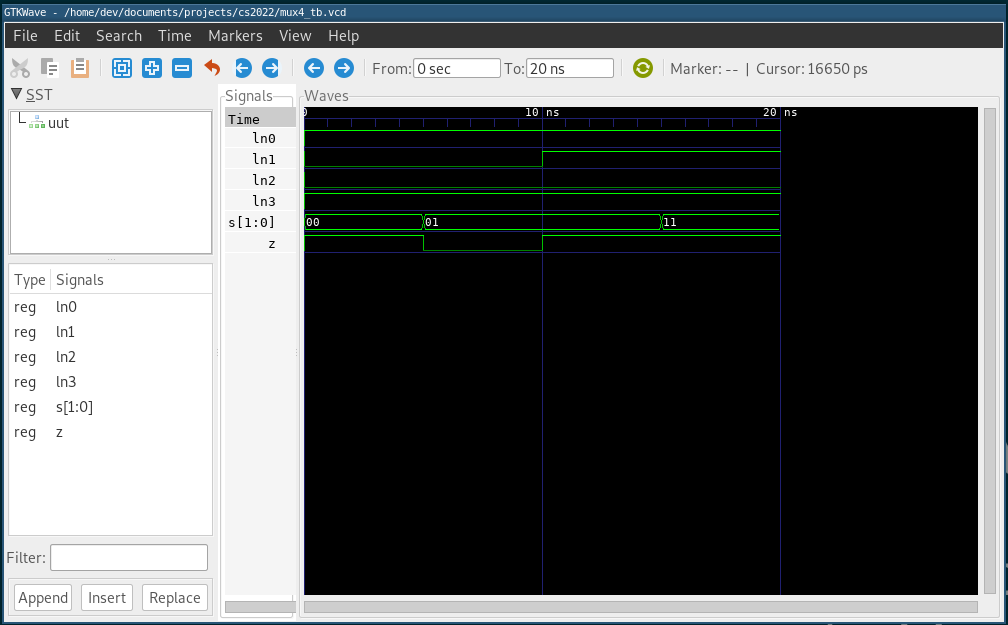
\includegraphics[width=\textwidth]{mux4_tb}
	\caption{\mi{c}{mux4} testbench results}
	\label{fig:mux4}
\end{figure}

Figure~\ref{fig:mux4} shows the simulation results of a simple 4-to-1 mux.
\begin{itemize}
	\item When \mi{c}{s = 00}, \mi{c}{z = 1} since \mi{c}{ln0 = 1}
	\item Changing \mi{c}{s = 01} results in \mi{c}{z = 0} as \mi{c}{ln1 = 0}
	\item Later \mi{c}{ln1 = 1}, at which point \mi{c}{z = 1}
	\item Finally, with \mi{c}{s = 11}, \mi{c}{z} remains the same since \mi{c}{ln3 = 1}
\end{itemize}

\emph{Note: testbenches for \mi{c}{mux2} and \mi{c}{mux3} were not included since they are simply 
reduced versions of \mi{c}{mux4}.}

\end{document}
# vim: nofoldenable
